\section{Project Overview} \label{Overview}

As stated in the introduction, the goal of our work is to implement a blockchain solution that can be used to fight frauds in the automotive world. To be more specific, we apply the ByzCoin \cite{ByzCoin Impl} blockchain technology and build a service on top of it.\\
\newline
For a correct implementation, the system requires at least 5 machines, with the assumption that at most one of them might be faulty or byzantine. This is deduced from the statement that ByzCoin tolerates $f$ faulty members among $3f + 2$ nodes in the system \cite{ByzCoin}. These conodes are envisioned to be distributed between the distrustful parties (car manufacturers and dealers, insurance companies, police...).\\
\newline
Each machine maintains a local copy of the blockchain and users are able to interact with the nodes by using a desktop application (Figure ~\ref{System Description}). They can either create and send a new transaction, or get a proof of existence for the data stored on the blockchain.
\begin{figure}[H]
    \centering
    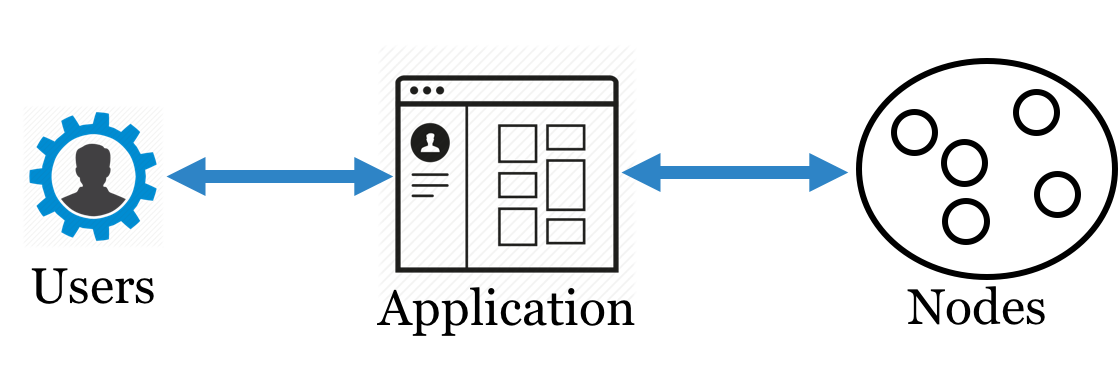
\includegraphics[width=0.75\textwidth]{Figures/system.png}
    \caption{System Description}
    \label{System Description}
\end{figure}
\noindent
In what follows, we describe the use case of our project.

\subsection{Use Case}

Depending on the access control in the system, blockchains can be public or private. Private blockchains are suitable only when a set of known players is allowed to participate. What ByzCoin and Calypso bring into the picture is the possibility to open the system to unknown participants.\\
\newline
Current limitation, which is not inherent to the system, is that an administrator, at the beginning, defines which conode machines are going to be part of the system and then sets the blockchain up. The administrator is also in charge of enrolling new cars and members, each time a new user decides to join the service. This accounts for a point of making profit, if registration charges are introduced.
\newline
There are several roles that the participants can take on (Figure ~\ref{Use Case Diagram}):
\begin{itemize}
    \item vehicle owner
    \item a person allowed to add maintenance reports (further on referred to as a garage mechanic)
    \item potential buyer
\end{itemize}
\vspace{10pt}
\begin{figure}[H]
    \centering
    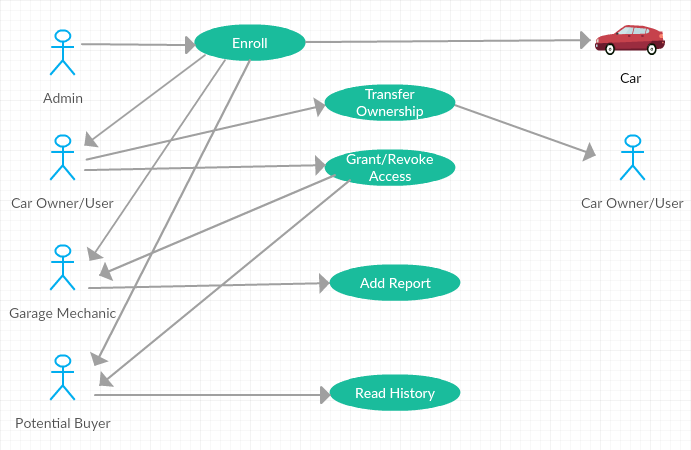
\includegraphics[width=1\textwidth]{Figures/use_case_diagram.png}
    \caption{Use Case Diagram}
    \label{Use Case Diagram}
\end{figure}
\vspace{10pt}
\noindent
The car owner is responsible for granting and revoking read access to potential buyers and write access to garage mechanics. Additionally, the ownership of the car history can easily be transferred to another user after a successful car sell without involving the administrator.\\ 
\newline
Furthermore, garage mechanics are responsible for data generation during every regular car inspection or unforeseen repair, and are also required to use the information provided by the IoT device connected to the car.\\
\newline
Finally, the entire maintenance history of the vehicles can be requested and read by the allowed potential buyers.\\
\newline
Having envisioned and described the system model, we are able to proceed with specifying the implementation details.


